
%------------------------------------------------------------------------
%
%    Copyright (C) 1985-2020  Georg Umgiesser
%
%    This file is part of SHYFEM.
%
%    SHYFEM is free software: you can redistribute it and/or modify
%    it under the terms of the GNU General Public License as published by
%    the Free Software Foundation, either version 3 of the License, or
%    (at your option) any later version.
%
%    SHYFEM is distributed in the hope that it will be useful,
%    but WITHOUT ANY WARRANTY; without even the implied warranty of
%    MERCHANTABILITY or FITNESS FOR A PARTICULAR PURPOSE. See the
%    GNU General Public License for more details.
%
%    You should have received a copy of the GNU General Public License
%    along with SHYFEM. Please see the file COPYING in the main directory.
%    If not, see <http://www.gnu.org/licenses/>.
%
%    Contributions to this file can be found below in the revision log.
%
%------------------------------------------------------------------------

The |grid| program allows one not only to visualize 
the |grd| files but provides also a graphical user interface 
to manipulate the different items of the grid (Nodes, Elements, Lines).

\begin{figure}[htbp]
\centering
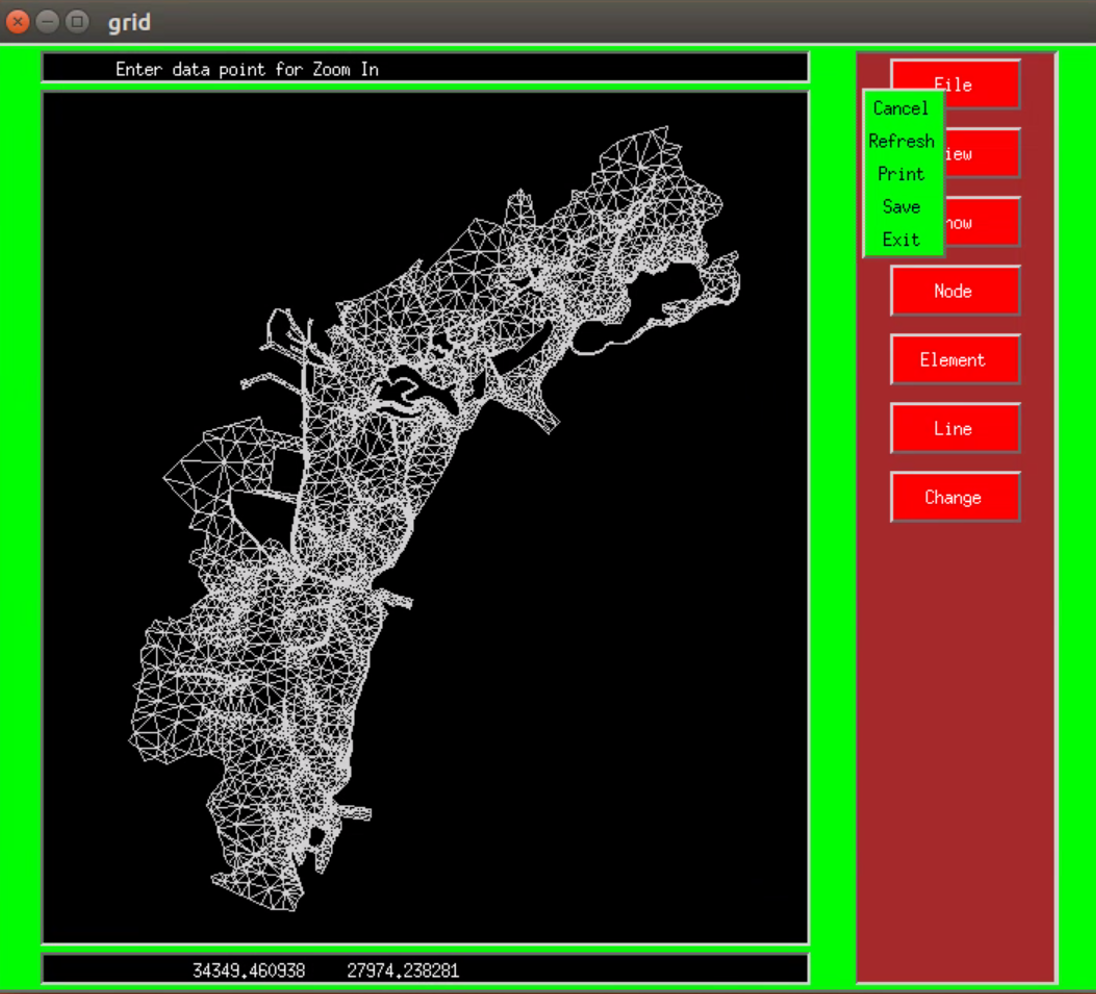
\includegraphics[scale=0.5]{grd.png}
\caption{Example of the GRD GUI provided in the model code}
\label{grd_gui}
\end{figure}

The command line and the options available for this program are reported below (and where those used in the procedure shown in \Fig\ref{line}).

\begin{verbatim}
grid [-options] [files] 

Options :
  -o   do not outline elements      -f   fill elements with color     
  -k   do extra checking            -u   check if nodes are used      
  -T   show type instead of depth   -c#  use color table #            
  -h   print this help screen       -a   ask for file names           
  -d   display  (only X11)          -g   geometry (only X11)          
  -M#  scale color to depth #       -S#  size of color table is #     
  -N#  scale factor for nodes is #  -V#  scale factor for vectors is #
  -C   color nodes and lines        -On  use n as output file name    
  -t#  use type # for new items
\end{verbatim}

\textbf{General GUI commands}

\descrpn{|scroll|}
\descrptext{%
zoom in and out
}
\par
\descrpn{|right click|}
\descrptext{%
select item
}
\par
\descrpn{|left click|}
\descrptext{%
confirm item
}
\par
\descrpn{|up arrow|}
\descrptext{%
increase the node size
}
\par
\descrpn{|down arrow|}
\descrptext{%
decrease the node size
}
\par

The main GUI menu is composed of

\descrpn{|File|}\par
\descrpn{|View|}\par
\descrpn{|Show|}\par
\descrpn{|Node|}\par
\descrpn{|Element|}\par
\descrpn{|Line|}\par
\descrpn{|Change|}\par

\textbf{File menu}

\descrpn{|Cancel|}
\descrptext{%
Obsolete command
}
\par
\descrpn{|Refresh|}
\descrptext{%
Refresh the screen view (to be done to view the last change to the grid)
}
\par
\descrpn{|Print|}
\descrptext{%
Create a Black and White PostScript of the grid |plot.ps|
}
\par
\descrpn{|Save|}
\descrptext{%
Save changes in |save.grd|
}
\par
\descrpn{|Exit|}
\descrptext{%
Quit GRID program
}
\par

\textbf{View menu}

\descrpn{|Zoom Window|}
\descrptext{%
Zoom in a delimited window defined by left clicking two points (left-bottom and right-top)  
}
\par
\descrpn{|Zoom in|}
\descrptext{%
Obsolete command replaced by mouse scroll
}
\par
\descrpn{|Zoom out|}\descrptext{%
Obsolete command replaced by mouse scroll
}
\par
\descrpn{|Total View|}
\descrptext{%
Go back to the total view of the grid
}
\par
\descrpn{|Move|}
\descrptext{%
Obsolete command
}
\par

\textbf{Show menu}

\descrpn{|Show Node|}
\descrptext{%
All the items selected by right clicking will be nodes
}
\par
\descrpn{|Show Element|}
\descrptext{%
All the items selected by right clicking will be elements
}
\par
\descrpn{|Show Line|}
\descrptext{%
All the items selected by right clicking will be lines
}
\par

\textbf{Node menu}

\descrpn{|Make Node|}
\descrptext{%
Create a new node by left clicking
}
\par
\descrpn{|Del Node|}
\descrptext{%
Delete a node by selecting it (right click) and confirming it (left click). |Refresh| to see the changes.
}
\par
\descrpn{|Move Node|}
\descrptext{%
Move a node in a new position. 
Select it (right click) and confirm it (left click), give the new position (left click). |Refresh| to see the changes.
}
\par
\descrpn{|Unify Node|}
\descrptext{%
Unify two different nodes. 
Select the first node you want to unify (right click) and confirm it (left click), select the second node (left click). |Refresh| to see the changes.
}
\par

\textbf{Element menu}

\descrpn{|Make Element|}
\descrptext{%
Create a new element.
Create new nodes (left click) or select and confirm (right-left click) each node of the new element, clicking twice on the last one to close the element. The element has to be created in anti-clockwise sense.
}
\par
\descrpn{|Del Element|}
Remove the element but not its nodes.
\descrptext{%

}
\par
\descrpn{|Remove Element|}
Remove the element and its nodes.
\descrptext{%

}
\par

\textbf{Line menu}

\descrpn{|Make Line|}
\descrptext{%
Create a new line.
Create new nodes (left click) or select and confirm (right-left click) each node of the new line, clicking twice on the last one. In case of a close line it has to be created in anti-clockwise sense.
}
\par
\descrpn{|Del Line|}
\descrptext{%
Remove the line but not its nodes.
}
\par
\descrpn{|Remove Line|}
\descrptext{%
Remove the line and its nodes.
}
\par
\descrpn{|Split Line|}
\descrptext{%
Split the line in two parts.
}
\par
\descrpn{|Join Line|}
\descrptext{%
Join two lines in one.
}
\par
\descrpn{|Del Node|}
\descrptext{%
Delete the node from line but not from the domain.
}
\par
\descrpn{|Remove Node|}
\descrptext{%
Remove the node from line.
}
\par
\descrpn{|Insert Node|}
\descrptext{%
Insert a new node on the line.
}
\par

\textbf{Change menu}

\descrpn{|Change Depth|}
\descrptext{%
Change the depth of the selected item.
}
\par
\descrpn{|Change Type|}
\descrptext{%
Change the type of the selected item.
}
\par






